% Chapter 10, Section 6

\section{Advanced Topics \difficultyInline{intermediate}}
\label{sec:rnn-advanced}

\subsection*{Intuition}

Variants extend context (bidirectional), depth (stacked layers), supervision signals (teacher forcing), and search quality (beam search). Beam search maintains multiple candidate sequences during generation, exploring promising paths rather than committing to a single greedy choice, which often leads to higher-quality outputs. These architectural and algorithmic choices create fundamental trade-offs that practitioners must navigate carefully. Training stability often comes at the cost of inference complexity, while improved context modeling may increase computational requirements. The optimal configuration depends heavily on the specific task requirements, available computational resources, and latency constraints. For example, real-time applications may prioritize speed over quality, while offline processing can afford more sophisticated search strategies. Understanding these trade-offs is crucial for designing effective RNN-based systems that meet both performance and practical deployment requirements.

\subsection*{Historical Context}

Bidirectional RNNs (BiRNN) emerged post-2000 as a key innovation to improve context use for labeling tasks like Part-of-Speech tagging. Instead of processing sequences unidirectionally, BiRNNs use two independent RNNs (often LSTMs): one running forward and one backward, with their outputs concatenated. This structure allows any element $x_t$ to benefit from both past and future context, resulting in much richer local context for classification. Teacher forcing stabilized decoder training but highlighted exposure bias; beam search became standard for autoregressive decoding in translation and speech.

% Index and glossary
\index{bidirectional RNN}
\index{teacher forcing}
\index{beam search}
\glsadd{attention-mechanism}

\subsection{Bidirectional RNNs}

The term "bidirectional" refers to processing the input sequence in both temporal directions—forward and backward—unlike standard RNNs that only process left-to-right. Mathematically, this means maintaining two separate hidden state sequences:

\begin{align}
\overrightarrow{\vect{h}}_t &= f(\vect{x}_t, \overrightarrow{\vect{h}}_{t-1}) \\
\overleftarrow{\vect{h}}_t &= f(\vect{x}_t, \overleftarrow{\vect{h}}_{t+1}) \\
\vect{h}_t &= [\overrightarrow{\vect{h}}_t; \overleftarrow{\vect{h}}_t]
\end{align}

The forward arrow $\overrightarrow{\vect{h}}_t$ processes the sequence from left to right (time $t-1$ to $t$), while the backward arrow $\overleftarrow{\vect{h}}_t$ processes from right to left (time $t+1$ to $t$). The final representation $\vect{h}_t$ concatenates both directions, giving each position access to both past and future context.

\paragraph{Metaphor.} Imagine reading a sentence twice: first normally from left to right to understand the flow, then reading it backward from right to left to catch any nuances you might have missed. A bidirectional RNN does exactly this—it "reads" the sequence in both directions simultaneously, allowing each word to be understood in the full context of what comes before and after it.

Useful when future context is available.

\paragraph{Use cases and caveats.} Effective for tagging, chunking, and ASR with full utterances, but not suitable for strictly causal, low-latency streaming since backward states require future tokens. Alternatives include limited-lookahead or online approximations.

\subsection{Deep RNNs}

Stack multiple RNN layers:
\begin{equation}
\vect{h}_t^{(l)} = f(\vect{h}_t^{(l-1)}, \vect{h}_{t-1}^{(l)})
\end{equation}

The term "deep" refers to the vertical stacking of multiple recurrent layers, where each layer $l$ processes the hidden states from the previous layer $l-1$ at each time step. This creates a hierarchical representation where lower layers capture local patterns and dependencies, while higher layers learn more complex, long-range temporal relationships. Unlike feedforward networks where depth refers to the number of layers, in deep RNNs, depth combines both the number of layers and the temporal dimension, creating a two-dimensional computational graph. Each layer can specialize in different aspects of the sequence modeling task, with early layers often focusing on local features and later layers integrating information across longer time horizons.

\paragraph{Visual aid.} Stacked recurrent layers over time.
\begin{figure}[h]
    \centering
    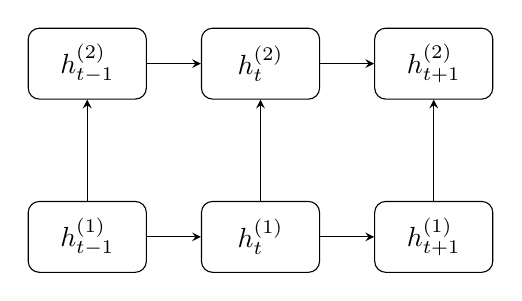
\begin{tikzpicture}[>=stealth, node distance=2.2cm]
        \tikzstyle{node}=[draw, rounded corners, minimum width=1.5cm, minimum height=0.9cm]
        % time t-1
        \node[node] (l1t1) {$\vect{h}_{t-1}^{(1)}$};
        \node[node, above of=l1t1] (l2t1) {$\vect{h}_{t-1}^{(2)}$};
        % time t
        \node[node, right of=l1t1] (l1t) {$\vect{h}_{t}^{(1)}$};
        \node[node, above of=l1t] (l2t) {$\vect{h}_{t}^{(2)}$};
        % time t+1
        \node[node, right of=l1t] (l1t2) {$\vect{h}_{t+1}^{(1)}$};
        \node[node, above of=l1t2] (l2t2) {$\vect{h}_{t+1}^{(2)}$};
        % horizontal
        \draw[->] (l1t1) -- (l1t);
        \draw[->] (l1t) -- (l1t2);
        \draw[->] (l2t1) -- (l2t);
        \draw[->] (l2t) -- (l2t2);
        % vertical
        \draw[->] (l1t1) -- (l2t1);
        \draw[->] (l1t) -- (l2t);
        \draw[->] (l1t2) -- (l2t2);
    \end{tikzpicture}
    \caption{Deep RNN: multiple recurrent layers stacked over time.}
\end{figure}

Practical tips: residual connections, layer normalization, and dropout between layers help optimization and generalization.

\subsection{Teacher Forcing}

During training, teacher forcing uses ground truth as the decoder input rather than the model's own predictions from the previous time step. This approach provides several significant advantages for training efficiency and stability. By providing the correct previous token during training, the model receives consistent, high-quality input signals that guide it toward the target distribution more directly, eliminating the compounding effect of early prediction errors that would otherwise propagate through the sequence and allowing the model to focus on learning the mapping from context to next token rather than recovering from its own mistakes. Teacher forcing ensures that each training step receives optimal input conditions, preventing the model from getting stuck in poor local minima caused by its own incorrect predictions, which creates a more predictable gradient landscape where the model can learn the underlying sequence patterns without being derailed by cascading errors.

However, teacher forcing introduces exposure bias at test time—a train–test mismatch where the model never learns to recover from its own errors. During training, the model only sees ground truth inputs, but at test time it must generate sequences using its own predictions, which may contain errors that compound over time, creating a distribution shift where the model's training experience doesn't match its inference conditions. Several mitigation strategies have been developed to address this issue, including scheduled sampling, where the model gradually transitions from using ground truth to its own predictions during training by probabilistically mixing the two, and sequence-level training objectives that optimise end-to-end sequence quality rather than individual token predictions, forcing the model to experience and adapt to its own prediction errors during training.
\glsadd{backpropagation}

\subsection{Beam Search}

For inference, beam search maintains the top-$k$ candidate hypotheses at each decoding step, offering substantial advantages over simpler decoding strategies. Greedy decoding always selects the single most probable token at each step, which can lead to suboptimal global sequences since locally optimal choices don't guarantee globally optimal solutions—the best next word when considered in isolation might not lead to the best complete sentence. Beam search explores multiple promising paths simultaneously, maintaining a "beam" of $k$ partial sequences ranked by their cumulative probability, which allows it to recover from early mistakes and find sequences with higher overall probability by considering how different choices affect the entire sequence quality.

The technique involves a fundamental trade-off between quality and computational cost. Larger beam sizes explore more hypotheses and generally produce higher-quality outputs, but require substantially more computation as the beam width increases, with computational cost growing as $O(k \times V)$ where $k$ is the beam size and $V$ is the vocabulary size, making very large beams impractical for real-time applications. Practitioners must carefully balance the quality improvement against the computational overhead, with typical beam sizes of 5–10 providing a good compromise for most applications. In neural machine translation systems, beam sizes are often combined with length normalisation—dividing sequence scores by their length to prevent the bias toward shorter sequences that naturally have higher probability scores—and coverage penalties that encourage the model to attend to all parts of the input sequence, ensuring all source words are translated. The specific beam size and normalisation strategy depend heavily on the task requirements, with more complex tasks often benefiting from larger beams and sophisticated scoring functions that incorporate domain-specific constraints.
